\documentclass{standalone}
\usepackage{tikz}
\usepackage{ctex,siunitx}
\setCJKmainfont{Noto Serif CJK SC}
\usepackage{tkz-euclide}
\usepackage{amsmath}
\usetikzlibrary{patterns, calc}
\usetikzlibrary {decorations.pathmorphing, decorations.pathreplacing, decorations.shapes,}

\begin{document}
\small
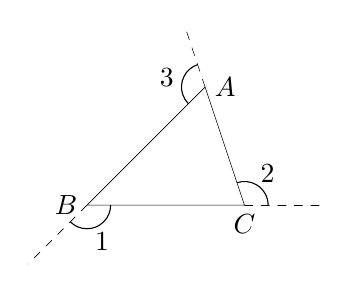
\begin{tikzpicture}[>=stealth,scale=1.0]
  \tkzSetUpPoint[fill=black]
  % \useasboundingbox(-1,-0.75)rectangle(3.7,1.4);
  \tkzDefPoints{0/0/B, 2/0/C, 1.5/1.5/A}
  \tkzDrawPolygon(A,B,C)
  \tkzDefPointWith[linear, K=1.5](C,A) \tkzGetPoint{A'}
  \tkzDefPointWith[linear, K=1.5](B,C) \tkzGetPoint{C'}
  \tkzDefPointWith[linear, K=1.5](A,B) \tkzGetPoint{B'}
  \tkzDrawSegments[dashed](A,A' B,B' C,C')
  \tkzLabelPoints[left](B)
  \tkzLabelPoints[right](A)
  \tkzLabelPoints[below](C)
  \tkzMarkAngles[mark=none, size=.3](B',B,C C',C,A A',A,B)
  \tkzLabelAngle[pos=.5](B',B,C){1}
  \tkzLabelAngle[pos=.5](C',C,A){2}
  \tkzLabelAngle[pos=.5](A',A,B){3}
\end{tikzpicture}
\end{document}